\chapter{Fejlesztői dokumentáció} % Developer guide
\label{ch:impl}




\section{Megvalósítási terv}

\subsection{Felhasználói felület}
\begin{figure}[H]
	\centering
	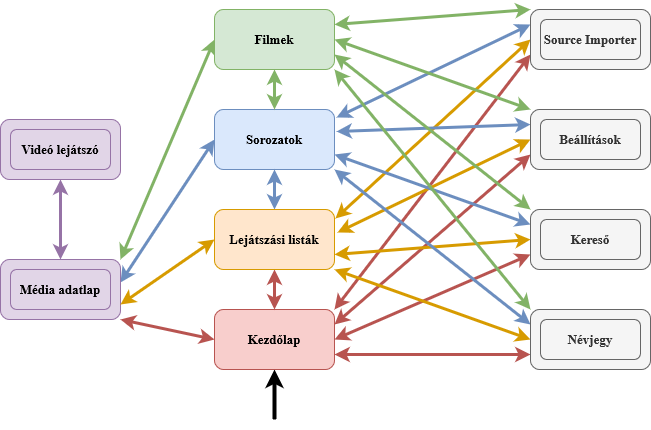
\includegraphics[width=1\textwidth]{navigation_between_screens.png}
	\caption{Navigáció az oldalak között}
	\label{fig:search}
\end{figure}

% ==========================================================
% |                    Implementáció                       |
% ==========================================================
\section{Implementáció}

\subsection{Használt technológiák}
Az alkalmazás fejlesztését JavaScript nyelven kezdtem meg és fejlesztés közben váltottam TypeScript nyelvre. A TypeScript gyakorlatilag egy típusos kiterjesztése a JavaScriptnek, éppen ezért minden kód amit JavaScriptben írtam azok érvényes és valid kódok TypeScriptben is. A TypeScript lényege, hogy típus biztossá teszi a kódot, ami megnehezíti a fejlesztést, de sok probléma már a fejlesztés során észlelhető - ezáltal javítható - és nem a kész verzióban történnek katasztrofális dolgok. Váltásom motivációja a TypeScript nyújtotta előnyök mellett az is volt, hogy az ipar jelenlegi trendjei teljesen efelé a nyelv felé mutatnak, minden komolyan vehető program már TypeScriptben íródik. Ez predesztinálta az én hozzáállásomat is a nyelvhez, tekintve hogy legelejétől fogva célom volt a legfrissebb és legnépszerűbb technológiák haszálata és ezen piacképes tudások elsajátítása.

\subsubsection{Electron}
Az Electron\footnote{\url{https://www.electronjs.org/}} egy nyílt forráskódú keretrendszer, amelyet asztali alkalmazások fejlesztéséhez lett kifejlesztve. Különlegessége, hogy webes technolgiákat lehet használni asztali alkalmazások fejlesztéséhez.

\subsubsection{React}

\subsubsection{Redux}

\subsection{Funkcionális megközelítés}

\section{Tesztelés}
